\begin{frame}
  \frametitle{\textbf{Phases of QCD}}
  \begin{itemize}
  \item For $\mathbf{\frac{\mu_B}{T} \leq 2}$, QGP-to-hadron phase transition is a \textbf{smooth crossover}
  \item Above some critical point, the QGP-to-hadron transition is expected to become a \textbf{first-order phase transition}
  \item Beam Energy Scan at RHIC $\to$ map the phase-diagram by varying $\mu_B$
  \end{itemize}

  \

  \centering

  \begin{columns}
    \column{0.65\textwidth}
    \begin{tikzpicture}
      \node{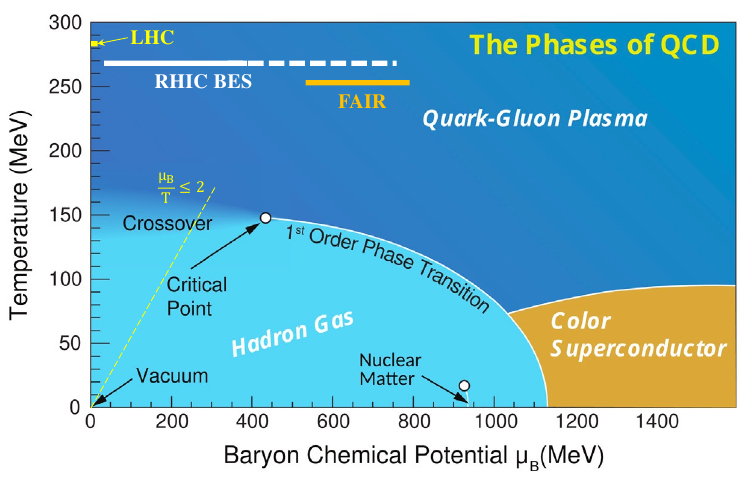
\includegraphics[width=\textwidth]{qcd-phase-diagram.png}};
      \node[font=\tiny,align=left] at (2.5,2.5) {\href{https://arxiv.org/abs/2303.17254}{arXiv:2303.17254}};
    \end{tikzpicture}
    \column{0.35\textwidth}
    \begin{tikzpicture}
      \node{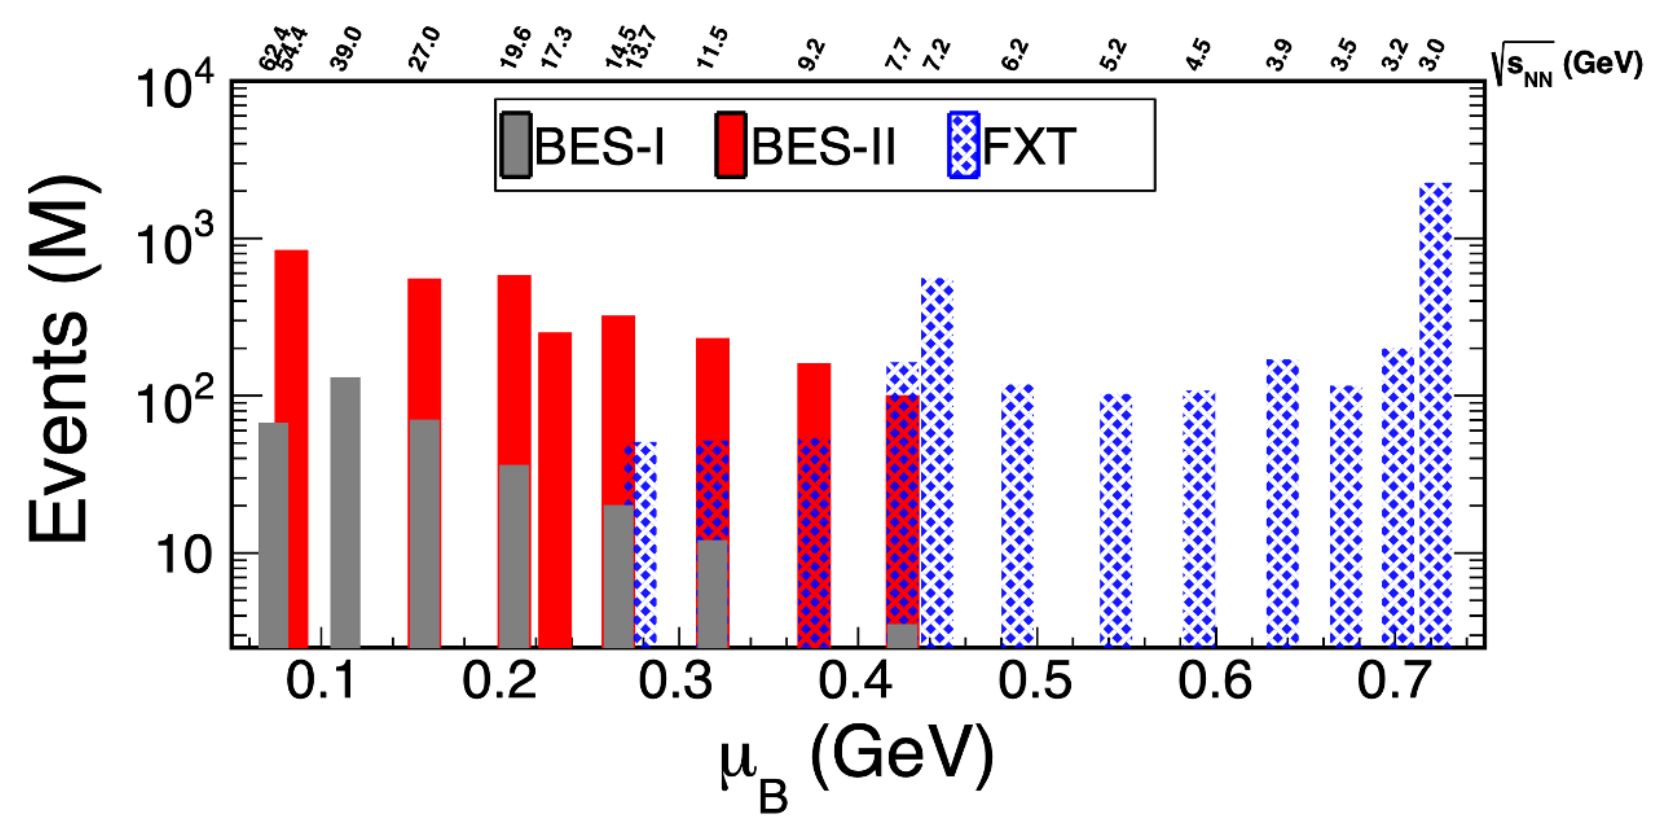
\includegraphics[width=\textwidth]{baryon-chemical-potential-BES.png}};
      \node[font=\tiny,align=left] at (1.,1.30) {$\boldmath{\mu_B}$ \textbf{from RHIC}};
    \end{tikzpicture}

    \
    \begin{columns}
    %  \column{0.55\textwidth}
    %\begin{tikzpicture}
    %  \node{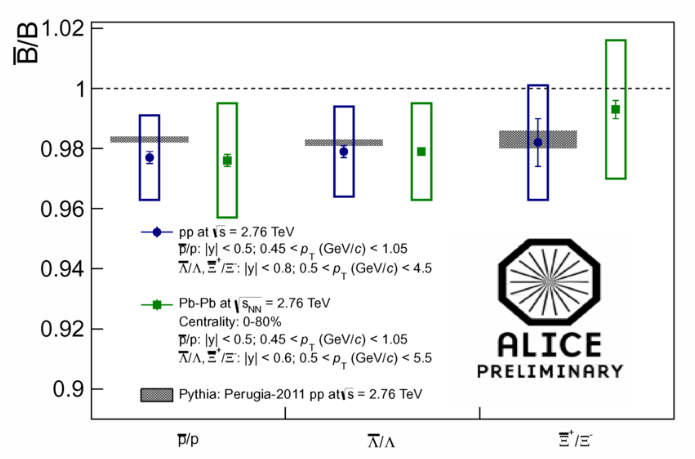
\includegraphics[width=\textwidth]{baryon-antibaryon-lhc.png}};
    %  \node[font=\tiny,align=left] at (0,1.0) {LHC: $\bar{p} / {p} \sim 1$};
    %\end{tikzpicture}
    \column{0.85\textwidth}
    \begin{tikzpicture}
      \node{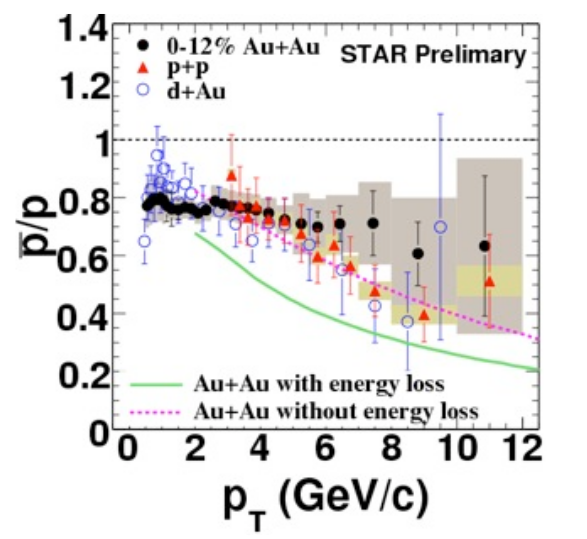
\includegraphics[width=\textwidth]{baryon-antibaryon-rhic.png}};
      \node[font=\tiny,align=left] at (0.2,1.7) {RHIC: $\bar{p} / p \sim 0.8$};
    \end{tikzpicture}
    \end{columns}
  \end{columns}
\end{frame}
